%!TEX root = ../plos_template.tex
\subsection{Intuitive description}\label{sec:intuition}
A genotype fundamentally determines a collection of interactions among genes. In this sense it is reasonable to consider a genotype to be a collection of subsets of genes, where the subsets encode the manner in which different genes interact with one another. These interactions result in phenotypes, which are observable properties that result from these interactions. At the most fundamental level, the phenotype is taken to be a measure of gene expression and in order to distinguish the possible phenotypes it is necessary to uniquely encode each expression state that corresponds to a given collection of interactions. For example, if we have three genes where all three genes interact with one another and each gene takes on one of two expression states, then our state space is determined by the $2^3$ binary sequences of length $3$. If instead of directly observing expression states, we observed a higher-level phenotype such as metabolite concentration, cell motility or shape, or in higher organisms even something as abstract as fur color, we could abstractly associate whatever number of labels are necessary to make all of the observable distinctions resulting in a model with an equivalent formalism.

A deterministic genotype-phenotype mapping is fundamentally a map from one set to another. As described above, we consider the input to be a collection of subsets of some set of genes that determine a genotype and the output to be a collection of abstract labels that are associated to a phenotype. The primary example of the phenotype labels used here assigns them to expression states of genes, but, to reiterate, the phenotype values can more generally be associated to other observable properties of organisms. The collection of all possible genotype-phenotype mappings corresponds to another set.

Different interactions among genes correspond to different ways of taking collections of subsets from the overall set of genes under consideration. So, the possible interactions among genes encoded in the collections of subsets that determine a particular genotype is included in the set of all genotype-phenotype mappings. Because of both the stochastic nature of the gene expression process and uncertainty in measurements of such, we do not generally consider a single genotype-phenotype map to constitute a model of the gene expression process. Instead, we assign a probability distribution over the entire collection of possible genotype-phenotype mappings. For the case in which a single genotype-phenotype map has probability 1, this method reduces to the deterministic case, so that it is not lost as a possibility in the generalization to include stochastic models.

Consideration of probability distributions on genotype-phenotype mappings where the genotype is a given collection of subsets of genes introduces an issue that must be dealt with in one manner or another both biologically and mathematically. From the biological perspective, genes involved in overlapping subsets must be able to function in one state or another in the context of multiple interactions. From the mathematical perspective, if the probability distributions over the mappings from subsets of genes to phenotype values is to be derived from a global mapping from all the genes included in the union of the subsets defining the genotype, then certain additional constraints that are not implicit in the simple normalization of probability distributions must be satisfied. The importance here of the so-called sheaf condition is that any collection of data that might represent contingency tables or marginal distributions must satisfy certain conditions in order to be able to be derived via the standard marginalization procedure from some joint distribution. Without satisfying these conditions, one may just have an incoherent collection of observations that could not have derived from any joint probability distribution.

The latter fact turns out to have an impact on the relationship between gene regulatory network architectures and their ability to achieve certain correlations among gene expression states and thus to perform certain functions. In order to quantify the relationships among the spaces of probability distributions over genotype-phenotype maps associated to each network architecture, we need to be able to determine the constraints associated to each network architecture and compare the geometries that result from imposing these constraints. In \ref{sec:dgpm} - \ref{sec:hierarchicalmodels} we describe the formalization of the stochastic genotype-phenotype map and the formal sheaf condition. In \ref{sec:example} - \ref{sec:generativeprocessapparentinconsistency} we provide an example computation used to derive the results presented in the main text. Readers primarily interested in the latter can skip to \ref{sec:example} and return to the earlier sections as needed.

\subsection{Deterministic genotype-phenotype maps}\label{sec:dgpm}
Consider the case in which we have a set of \emph{genes} $L$ indexed by $i=1, \ldots, m$. A subset of genes will be denoted as $U \subseteq L$. We also have a set of phenotypes $P$. In principle, any gene could give rise to any phenotype. A genotype-phenotype map is thus represented as a function mapping a subset of genes into phenotypes\footnote{In the operationalist framework from which this modeling description derives \cite{Abramsky2011}, our genes and subsets thereof $U \subseteq L$ are analogous to measurements and subsets thereof $T \subseteq X$ and our phenotypes $P$ are like measurement outcomes or values $V$. An event in which outcomes $s(t)$ are observed for each $t \in T$ serve to define mappings called \emph{sections} over $T$ as $s \colon T \rightarrow V$.}
$$
e \colon U \rightarrow  P.
$$

We denote the set of all subsets of a set $X$ as $\mathcal{P}(X)$. $\mathcal{P}(L)$ can then be viewed as a category~\cite{Lane1998,MacLane1992,Awodey2006} in which the objects are subsets of genes and morphisms represent inclusion of a smaller subset into a larger superset (i.e. $U \subseteq U' \Rightarrow U \rightarrow U'$). The category $\mathcal{P}(L)^{opp}$ then has the same objects, but the morphisms represent restriction from a larger to a smaller subset of genes (i.e. $U' \supseteq U \Rightarrow U' \rightarrow U$). In order to consider the set of all genotype-phenotype maps, for a given set of genes $L$, together, we can construct a functor
$$
\mathcal{E} \colon \mathcal{P}(L)^{opp} \rightarrow Set
$$
by exhibiting precisely how it acts on objects and morphisms in its domain category. We explicitly represent the way in which the functor $\mathcal{E}$ acts on objects $U$ and morphisms $U \subseteq U'$ respectively as
\begin{equation}\label{eq:gpfunctor}
\begin{split}
\mathcal{E} \colon \mathcal{P}(L)^{opp} &\rightarrow Set,\\
U &\mapsto P^U,\\
U \subseteq U' &\mapsto res^{U'}_{U}.
\end{split}
\end{equation}
So the functor $\mathcal{E}$ takes a subset of genes and returns the set of genotype-phenotype mappings from the given subset of genes to the set of phenotypes. The restriction map operates on sets deriving from the application of $\mathcal{E}$ to a subset of genes as follows
\begin{eqnarray*}
res^{U'}_{U} \colon \mathcal{E}(U') &\rightarrow& \mathcal{E}(U)\\
P^{U'} &\rightarrow& P^U\\
e' \colon U' \rightarrow P &\mapsto& e'|_U \colon U \rightarrow P
\end{eqnarray*}
$\mathcal{E}$ is thus, by definition, a presheaf functor, which is an object in the functor category $Sets^{\mathcal{P}(L)^{opp}}$.

\subsection{Stochastic genotype-phenotype maps}\label{sec:sgpm}
There may be several sources for stochasticity in genotype-phenotype mapping including small numbers of the causal molecules and products of gene expression as well as environmental fluctuations upon which genotype-phenotype mappings are conditioned \cite{Swain2002,Paulsson2004,Thattai2004,Acar2008a,Lestas2010,Munsky2012,Chalancon2012,Neuert2013,Sanchez2013}. Regardless of the fundamental nature of stochasticity to gene expression, empirically, we observe statistical as opposed to deterministic data. Here we generalize the deterministic framework outlined above to the stochastic case.

An \emph{algebraic structure} is determined by a set and one or more finitary operations (e.g. binary multiplication) defined on the elements of that set \cite{PachterLior2005,Artin2010}. A \emph{monoid} is a type of algebraic structure determined by a set and a binary operation such that the latter satisfies closure, associativity and identity with respect to the given set. A \emph{semiring} is an algebraic structure determined by a set with two binary operations. One of the binary operations, addition, forms a commutative monoid and has identity element 0. The second binary operation, multiplication, is a monoid with identity element 1. These binary operations interact such that multiplication distributes over addition and multiplication by the identity element of the addition monoid annihilates all elements in the semiring. For example, the real numbers under addition and multiplication constitute a semiring whose data is described as $\left( \mathbb{R},+,0,\times,1 \right)$.

Consider a function, $\phi$ from a set, $L$, to a semiring $R$ written $\phi \colon L \rightarrow R$. The \emph{support} of $\phi$, $\text{supp}(\phi)$, is then the set $\{ l \in L | \phi(l) \neq 0 \}$. A distribution, $d$, with respect to the semiring $R$ on $L$ is given as a function having finite support and satisfying a constraint
\begin{eqnarray*}
d \colon L \rightarrow R,\\
\sum_{l \in L} d(l) = 1
\end{eqnarray*}
We can consider the set of all distributions with respect to a given semiring $R$ satisfying the above constraints and defined on the set $L$ as being given by a functor applied to $L$ as $\mathcal{D}_R (L)$. We can again explicitly represent the way in which the functor $\mathcal{D}_R$ acts on objects and morphisms $L$ and $f \colon L \rightarrow M$ (where $L$ and $M$ are sets viewed as sets of genes and in some special cases we may have $M=L$) as
\begin{equation}\label{eq:distfunctor}
\begin{split}
\mathcal{D}_R \colon Set &\rightarrow Set,\\
L &\mapsto \mathcal{D}_R (L),\\
f \colon L \rightarrow M &\mapsto \mathcal{D}_R (f) \colon \mathcal{D}_R (L) \rightarrow \mathcal{D}_R (M),
\end{split}
\end{equation}
where
\begin{eqnarray*}
\mathcal{D}_R (f) \colon \mathcal{D}_R (L) &\rightarrow& \mathcal{D}_R (M),\\
d &\mapsto& \left[ m \mapsto \sum_{f(l)=m} d(l) \right].
\end{eqnarray*}
For the case in which we consider $R$ to be the semiring of non-negative real numbers $\left( \mathbb{R}_{\geq 0},+,0,\times,1 \right)$, $\mathcal{D}_R (L)$ represents the set of probability distributions over the set $L$.

Recalling the presheaf functor, $\mathcal{E} \colon \mathcal{P}(L)^{opp} \rightarrow Set$, mapping genotypes to the set of maps from those genotypes to the set of phenotypes, we can now compose it with the distribution functor $\mathcal{D}_R$ to obtain a new presheaf functor $\mathcal{D}_R \circ \mathcal{E} \colon \mathcal{P}(L)^{opp} \rightarrow Set \rightarrow Set$ that assigns to each genotype a distribution over the set of maps from those genotypes to the set of possible phenotypes. The action of $\mathcal{D}_R \mathcal{E}$ on objects and morphisms in $\mathcal{P}(L)^{opp}$ yields
\begin{eqnarray*}
\mathcal{D}_R \mathcal{E} \colon \mathcal{P}(L)^{opp} &\rightarrow& Set,\\
U &\mapsto& \mathcal{D}_R \mathcal{E}(U) \equiv d \colon P^U \rightarrow R,\\
U \subseteq U' &\mapsto& \mathcal{D}_R \mathcal{E}(U') \rightarrow \mathcal{D}_R \mathcal{E}(U).
\end{eqnarray*}
where
\begin{eqnarray*}
\mathcal{D}_R \mathcal{E}(U') &\rightarrow& \mathcal{D}_R \mathcal{E}(U),\\
d \colon P^{U'} \rightarrow R &\rightarrow& d|U \colon P^{U} \rightarrow R
\end{eqnarray*}
and
\begin{eqnarray*}
d \colon P^{U'} &\rightarrow& R,\\
s' &\mapsto& d(s');\\
d|U \colon P^{U} &\rightarrow& R,\\
s &\mapsto& \sum_{s' \in \mathcal{E}(U'),\, s'|U=s} d(s').
\end{eqnarray*}
$d|U$ is a representation of what is commonly referred to as the marginal distribution of $d$ that assigns to each genotype-phenotype mapping in the smaller collection (recall $U \subseteq U'$) of such $P^{U}$ the sum of the probabilities of all genotype-phenotype maps in the larger collection $P^{U'}$ that restrict to a given map in $P^{U}$.

\subsection{Coverings of genotype space}\label{sec:covergenotypespace}
A \emph{gene regulatory network module} is represented by a subset of genes $O$ and a collection of gene regulatory network modules, which in some cases may represent all of the genes in an organism, is a set of such subsets $\mathcal{G}$ (i.e. $O,O',\ldots \in \mathcal{G}$). An individual may be composed of some collection of subsets of possible genes where the set of all genes, $L$, is viewed as the genotype space. A \emph{covering} of the genotype space, $\mathcal{G}$, satisfies 1. $\cup_i O_i = \cup \mathcal{G} = L$ and 2. if $O,O' \in \mathcal{G}$ and $O \subseteq O'$ means that $O = O'$. This is equivalent to $\mathcal{G}$ being a reduced hypergraph , Sperner family or clutter \cite{Lauritzen1996}. The first condition means that $\mathcal{G}$ covers $L$. It is thereby just a statement that $\mathcal{G}$ represents a decomposition of the collection of all genes under consideration into subsets and this is why we refer to $\mathcal{G}$ as a collection of gene regulatory network modules. The second condition means simply that we will not consider nested subsets and so we will take for our $O \in \mathcal{G}$ the biggest $O \in \mathcal{G}$ that is not a subset of some other $O' \in \mathcal{G}$. The second condition also implies that if a given subset of genes $O'$ is compatible in a sense to be explained more precisely in what proceeds then any smaller subset of genes $O$ is also compatible. Coverings $\mathcal{G}$ of the genotype space contain the necessary information to make precise what we heuristically refer to at other points in this paper as modularity in order to cohere with standard terminology in systems biology literature while attempting to submit our own precise interpretation of the relatively colloquial concept.

\subsection{Compatibility of distributions on genotype-phenotype maps}\label{sec:compatibilityofgpms}
Given a covering of the genotype space $\mathcal{G}$, a compatible family for $\mathcal{G}$ with respect to the distribution presheaf $\mathcal{D}_R\mathcal{E}$ is given by a family of distributions $\{d_O \colon P^O \rightarrow R | O \in \mathcal{G}\}$ such that for all $O \in \mathcal{G}$ there exists $d_O \in \mathcal{D}_R\mathcal{E}(O)$ such that for all $O' \in \mathcal{G}$
\begin{eqnarray}\label{eq:sheafcond}
%\forall O \in \mathcal{G} \left[ \exists d_O \in \mathcal{D}_R\mathcal{E}(O) \right],\\
d_O|O \cap O' = d_{O'}|O \cap O'.
\end{eqnarray}
The condition \ref{eq:sheafcond} is referred to as the \emph{sheaf condition}. This condition means that any two distributions $d_O$ and $d_{O'}$ in the \emph{compatible family} of distributions produce the same values in the semiring $R$ on all of the genes in the intersection of $O$ with $O'$.

For example, if we have two gene regulatory network modules given by their genotypes $O = \{l_1, l_2\}$ and $O' = \{l_1, l_3\}$ then the sheaf condition specifies that for $e_{\{l_1\}} \in \mathcal{E}(\{l_1\})$, which assigns a particular phenotype to the genotype $\{l_1\}$ rather than to an entire gene regulatory network module like $O$ or $O'$, that
\begin{eqnarray}\label{eq:sheafprob}
\sum_{e \in \mathcal{E}(O),\, e|l_1=e_{\{l_1\}}} d_O(e) \,\, = \sum_{e' \in \mathcal{E}(O'),\, e'|l_1=e_{\{l_1\}}} d_{O'}(e')
\end{eqnarray}
This condition means that the probability for gene $l_1$ to be associated to the phenotype given by $e_{\{l_1\}}$ is equivalent in case we marginalize over all the other genes contained in the gene regulatory network modules of which $l_1$ is a component. For coherence with respect to the relationship between the modeling framework described here and that used in probabilistic graphical models in machine learning, the conditions \ref{eq:sheafprob} are referred to as the marginalization constraints \cite{Wainwright2007}.

\subsection{Global sections of distributions over genotype-phenotype maps}\label{sec:globalsectiongpms}
To say that the sheaf condition holds for a compatible family $\{d_O\}_{O \in \mathcal{G}}$ for the presheaf $\mathcal{D}_R\mathcal{E}$ implies the existence of a \emph{global section} $d \in \mathcal{D}_R\mathcal{E}(L)$ that is defined on the full set of genes. An example of a distribution that could be a global section given that it satisfies the sheaf condition is shown in \ref{tab:hidvarmod}. This global section defines a distribution on the set of genotype-phenotype maps given by $\mathcal{E}(L) = P^L$, specifying phenotypes associated to all genes at once instead of on subsets of $L$ associated to either $U \subseteq L$ or, what is essentially equivalent, $O \in \mathcal{G}$. Crucially, the distribution $d$ must also restrict for the subset of genes associated to any gene regulatory network module, which in some cases may represent all of the genes in an organism, $O$ in a covering of the genotype space $\mathcal{G}$ meaning that
\begin{eqnarray}
\forall O \in \mathcal{G} \left[ d|O = d_O \right].
\end{eqnarray}
In terms of distributions, the existence of a global section $d$ for a covering of the genotype space $\mathcal{G}$ corresponds to the existence of a distribution defined on all genes that marginalizes to yield the distributions on subsets of genes that may be observed empirically.

The presheaf $\mathcal{E}$ alone was already a sheaf because given a cover $\{U_i\}_{i \in I}$ of $U$ there is a family of sections $\{e_i \in \mathcal{E}(U_i)\}_{i \in I}$ that is compatible in the sense that
\begin{eqnarray}
\forall i,j \in I \left[ e_i|U_i \cap U_j = e_j|U_i \cap U_j \right].
\end{eqnarray}
In this case there is a unique global section $e \in \mathcal{E}(U)$ such that $\forall i \in I \left[ e|U_i = e_i \right]$. The fact that the sheaf condition holds for $\mathcal{E}$ is true because we are considering functions defined on a space with a trivial discrete topology allowing us to combine any partial functions that agree on overlapping subsets by taking the union of the data defining such functions.

Extending this example on an arbitrary subset $U \subseteq L$ to the whole set of genes $L$ we have a unique global section $e \in \mathcal{E}(L) = P^L$. $e$ can be used to deterministically assign phenotypes to the set of genes $L$ under consideration.

\subsection{Hierarchical models}\label{sec:hierarchicalmodels}
Given the collection of mappings $\mathcal{E}(O) = P^O$ for all $O \in \mathcal{G}$ we can attempt to explicitly construct a particular joint probability distribution $s \in \mathcal{D}_{\mathbb{R}}\mathcal{E}(L)$ on $\mathcal{E}(L)$. As noted above, in some cases such as that of \ref{fig:inconsistentthreecycle}A and C, such attempts may fail. This requires, first, a choice of mapping $\mathbb{R}^{\mathcal{E}(L)} \rightarrow \mathcal{D}_{\mathbb{R}}\mathcal{E}(L)$, which in the case of so-called \emph{exponential families} is
\begin{eqnarray*}
\text{exp} \colon \mathbb{R}^{\mathcal{E}(L)} &\rightarrow& \mathcal{D}_{\mathbb{R}}\mathcal{E}(L),\\
g &\mapsto& \frac{e^g}{\sum_{d \in \mathcal{E}(L)} e^{g(d)}}.
\end{eqnarray*}
In this case the exponential family is the image $exp(\mathcal{I}) \subset \mathcal{D}_{\mathbb{R}}\mathcal{E}(L)$ where $\mathcal{I} \subseteq \mathbb{R}^{\mathcal{E}(L)}$.

Given $\mathcal{G}$ we can associate an interaction subspace
$$
\mathcal{I}_{O} = \{ g \in \mathbb{R}^{\mathcal{E}(L)}\,\, |\,\, g(d_O,d_{L \setminus O}) = g(d_O,d'_{L \setminus O}) \text{ for all } d_O \in \mathcal{E}(O) \text{ and } d_{L \setminus O},d'_{L \setminus O} \in \mathcal{E}(L \setminus O)\}
$$
to each $O \in \mathcal{G}$. We can then construct the space of interactions associated to $\mathcal{G}$ itself as the sum over each interaction subspace
$$
\mathcal{I}_{\mathcal{G}} = \sum_{O \in \mathcal{G}} \mathcal{I}_{O}.
$$
The \emph{hierarchical model} \cite{Lauritzen1996} associated to $\mathcal{G}$ is then the exponential family
$$
\mathcal{E}xp_{\mathcal{G}} = \text{exp}(\mathcal{I}_{\mathcal{G}}).
$$
Markov random fields in the context of probabilistic graphical models or just graphical models are special cases of hierarchical models \cite{Lauritzen1996,Murphy2012}. In the main text, we use this notion in the numerical simulations to generate \ref{fig:inconsistentthreecycle}. Our reduced hypergraphs which correspond to GRNAs modeled as coverings of the collection of genes correspond more closely to what is referred to in machine learning as \emph{factor graphs} \cite{Barber2012,Bishop2007,Murphy2012,Koller2009}. The description in this section is taken from \cite{Lauritzen1996}, which uses hypergraphs explicitly.

\subsection{Example}\label{sec:example}
We can construct an example to make the model description more concrete. For this example, we take the full set of potential genes to be $L = \{ l_1,l_2,l_3,l_4 \}$. Consider the case in which each of the gene regulatory network modules under consideration has two genes and we specify the covering of the genotype space given by $\mathcal{G} = \{\{l_1,l_2 \},\{l_1,l_4 \},\{l_3,l_2\},\{l_3,l_4\} \}$. The full set of genes together with a covering of the genotype space is a special case of a hypergraph $\mathcal{H} = (L,\mathcal{G})$ where the set of genes $L$ serve as the nodes or vertices and the covering $\mathcal{G}$ contains the edges or hyperedges, each of which is simply some subset of $L$. We also have two phenotype values $P = \{0, 1\}$. Each genotype-phenotype map in \ref{tab:gpm} assigns phenotype values to each $O \in \mathcal{G}$. For example, $e_1 \colon   l_1 l_2 \rightarrow 00$. \ref{tab:probabilities} likewise assigns probabilities to each of these genotype-phenotype mappings.

We can collect all of these genotype-phenotype mappings into one set using \ref{eq:gpfunctor} as $\mathcal{E}(\mathcal{G}) = P^{\mathcal{G}} = \{e_i | i=1 \ldots 16 \}$. The operation $\mathcal{D}_R$ given in \ref{eq:distfunctor} converts the set of all possible genotype-phenotype maps into the set of probability distributions over that set of possible genotype-phenotype maps. Successively applying these operations yields a distribution function $\mathcal{D}_R\mathcal{E}(\mathcal{G})=d \colon P^\mathcal{G} \rightarrow R$. If we now apply this distribution function $d$ to the set of genotype-phenotype mappings we get the probabilities associated to each genotype-phenotype map $d(\{e_i | i=1 \ldots 16 \}) = \{p_i|i=1 \ldots 16\}$ given in \ref{tab:probabilities}. This can also be written more abstractly as $\left[\mathcal{D}_R\mathcal{E}(\mathcal{G})\right](\{e_i | i=1 \ldots 16 \}) = \left[\mathcal{D}_R\mathcal{E}(\mathcal{G})\right](P^\mathcal{G}) = \left[\mathcal{D}_R\mathcal{E}(\mathcal{G})\right](\mathcal{E}(\mathcal{G})) = \{p_i|i=1 \ldots 16\}$. Notice that we applied the operations $\mathcal{E}$ and $\mathcal{D}_R$ to a specific set, which was all of $\mathcal{G}$. We could have applied these operations to any $O \in \mathcal{G}$. In one case, for example if we take $O = \{l_1, l_2\}$, we would have gotten $\mathcal{E}(O) = \{e_i|i=1 \ldots 4\}$ and $\mathcal{D}_R\mathcal{E}(O) = d \colon P^O \rightarrow R$. In this case $\left[\mathcal{D}_R\mathcal{E}(O)\right](\mathcal{E}(O)) = \{p_i|i=1 \ldots 4\}$. We may even consider directly the meaning of $\left[\mathcal{D}_R\mathcal{E}(\{l_1\})\right](\mathcal{E}(\{l_1\}))$ and similarly for the other $l \in L$ for those subsets containing only one element of $L$.

Once we start considering probability distributions on subsets of $L$, we must introduce certain constraints to ensure that those probability distributions indeed derive from some probability distribution on the whole set $L$.  The sheaf condition then introduces a system of equations relating and thus constraining the probability parameters, beyond the constraint that each independently sum to one. The importance here of the sheaf condition is that any collection of data that might represent contingency tables or marginal distributions must satisfy certain conditions in order to be able to be derived via the standard marginalization procedure from some joint distribution. Without satisfying these conditions, one may just have an incoherent collection of observations that could not have derived from any joint probability distribution.  The constraint introduced by the sheaf condition is expressed in \ref{eq:sheafprob}, specialized to this example by
\begin{eqnarray}\label{eq:sheafprob2}
\sum_{e \in \mathcal{E}(\{l\}),\, e|l=e_{\{l\}}} d_{\{l\}}(e) \,\, = \sum_{e \in \mathcal{E}(O),\, e|l=e_{\{l\}}} d_O(e) \,\, = \sum_{e' \in \mathcal{E}(O'),\, e'|l=e_{\{l\}}} d_{O'}(e'),
\end{eqnarray}
for each $l \in L$, $e_{\{l\}} \in \mathcal{E}(\{l\})$, and $\{O \in \mathcal{G}|l=o, o \in O\}$. The resulting equations are explicitly indicated in like colors between the columns of \ref{tab:sheaf} :
\begin{equation}
\begin{aligned}\label{eq:pparsys}
p^*_1 &= p_1 + p_3 = p_5 + p_7, &
p^*_2 &= p_2 + p_4 = p_6 + p_8,\\
p^*_3 &= p_9 + p_{11} = p_{13} + p_{15},&
p^*_4 &= p_{10} + p_{12} = p_{14} + p_{16},\\
p^*_5 &= p_1 + p_2 = p_9 + p_{10},&
p^*_6 &= p_3 + p_4 = p_{11} + p_{12},\\
p^*_7 &= p_5 + p_6 = p_{13} + p_{14},&
p^*_8 &= p_7 + p_8 = p_{15} + p_{16}.
\end{aligned}
\end{equation}

Consider the meaning of the sheaf condition for $\mathcal{D}_R\mathcal{E}(L)$. $d \in \mathcal{D}_R\mathcal{E}(L)$ specifies a distribution whose domain consists of deterministic functions $\mathcal{E}(L) = P^L$ that map each gene independently, and independent of the fact that some combinations of genes  comprise gene regulatory network modules consisting of potentially interacting genes, to a phenotype. Since we have stated that $\mathcal{E}(L)$ satisfies the sheaf condition, for a given covering of the genotype space, $\mathcal{G}$, a globally compatible function $e \in  \mathcal{E}(L)$ restricts to $e|O$ for each $O \in \mathcal{G}$ such that there is a tuple of phenotypes assigned to genes that participate in overlapping gene regulatory network modules. Each $e \in P^L$ is associated to a trivial distribution $\delta_e \in \mathcal{D}_R\mathcal{E}(L)$ such that
\begin{eqnarray}
\delta_e(e') =
\begin{cases}
1, & e' = e,\\
0, & e' \neq e.
\end{cases}
\end{eqnarray}
For each gene regulatory network module $O$ we note that $\delta_e|O = \delta_{e|O}$. In this case, we can write the empirically determined distribution such as \ref{tab:probabilities} for a particular gene regulatory network module $d_O$ in terms of the distribution defined on the global set of genes restricted to a particular gene regulatory network module $d|O$:
\begin{equation}\label{eq:factordist}
\begin{split}
d_O(e) &= d|O(e)\\
&= \sum_{e' \in \mathcal{E}(L),e'|O=e} d(e')\\
&= \sum_{e' \in \mathcal{E}(L)} \delta_{e'|O}(e) \, d(e') = \sum_{e' \in \mathcal{E}(L)} \delta_{e'}|O(e) \, d(e')
\end{split}
\end{equation}
where
\begin{equation*}
\delta_{e'}|O(e) = \prod_{o \in O} \delta_{e'|\{o\}}(e|\{o\}).
\end{equation*}
We recover the empirically determined distribution as a sum over the deterministic genotype-phenotype mappings weighted by the probabilities of the distribution $d \in \mathcal{D}_R\mathcal{E}(L)$ defined over the full set of such deterministic mappings.

Thus, when there is a global section, given by $d \in \mathcal{D}_R\mathcal{E}(L)$, for an empirically determined distribution on genotype-phenotype mappings, for example that in \ref{tab:probabilities}, then it may be the case that a mechanism that stochastically selects among deterministic genotype-phenotype maps can satisfy or generate an empirically determined distribution.

\subsection{Existence of a global section for an empirically determined distribution of genotype-phenotype mappings}\label{sec:globalsectionempirical}
Given an empirically determined distribution on the genotype-phenotype mapping process, it may be helpful to be able to classify whether or not there exists a global section satisfying the sheaf condition in order to determine the modularity requirements of the empirical distribution. If an empirically determined distribution does have a global section, then it is possible to achieve the same global biological function specified in the empirical distribution using a single gene regulatory network module that contains all of the genes in the given universal set of genes $L$ as is obtained using the particular cover of the genotype space $\mathcal{G}$ that is associated to the empirically determined distribution. If the empirically determined distribution does not have a global section satisfying the sheaf condition, then there is some contingency regarding interactions between genes necessitating decomposition into smaller submodules than is represented by the whole of the universal set of genes $L$.

For a cover of the genotype space, $\mathcal{G}$, we can construct an incidence matrix, $\mathbf{G}$, representing the relationship between genotype-phenotype mappings having as domain particular gene regulatory network module contexts given by the $O \in \mathcal{G}$ and those global genotype-phenotype mappings defined on $L$. This is equivalent to the more formal statement that there is some binary relation,
\begin{equation}
R \subseteq \mathcal{E}(L) \times \coprod_{O \in \mathcal{G}} \mathcal{E}(O),
\end{equation}
whose \href{http://en.wikipedia.org/wiki/Logical_matrix#Matrix_representation_of_a_relation}{logical matrix representation}, $\mathbf{G}$, we would like to construct. In the first case, $\mathcal{E}(L) = P^L$ we have $\{t_1, \ldots t_m\} = \{t_j | t_j \in P^L\}$. In the second case, $\coprod_{O \in \mathcal{G}} \mathcal{E}(O)$, we have $\{e_1, \ldots e_n\} = \coprod_{O \in \mathcal{G}} \mathcal{E}(O)$. So we have two sets of maps, one defined on $P^L$ and the other defined on $\mathcal{E}(O) = P^O$ for each $O \in \mathcal{G}$. This yields a method of specifying the intended relationship that defines $\mathbf{G}_{n \times m}$ in terms of $t_j \in P^L$ and $e_i \in \mathcal{E}(O)$ :
\begin{eqnarray}
\mathbf{G}[i,j] =
\begin{cases}
1, & t_j|O = e_i,\\
0, & \text{otherwise}.
\end{cases}
\end{eqnarray}
This matrix can be viewed as an operator acting via matrix multiplication on distributions
\begin{eqnarray*}
\mathbf{G} \colon \mathcal{D}_R\mathcal{E}(L) &\rightarrow& \mathcal{D}_R\mathcal{E}(\mathcal{G}),\\
d &\mapsto& (d|O)_{O \in \mathcal{G}},
\end{eqnarray*}
and thereby taking a global distribution defined on genotype-phenotype maps whose domain is the full set of genes $L$ to the \emph{marginalized} distributions that are defined relative to gene regulatory network modules contained in a covering of the genotype space $\mathcal{G}$. This is to say that $\mathbf{G} \cdot d = (d|O)_{O \in \mathcal{G}} = \{d_O\}_{O \in \mathcal{G}}$. $\mathbf{G}$ provides a way of determining the kinds of environmentally determined distributions on genotype-phenotype mapping (i.e. $\{d_O\}_{O \in \mathcal{G}}$, \ref{tab:probabilities}) that can be derived from distributions (i.e. $\mathcal{D}_R \mathcal{E}(L)$) defined on the global genotype-phenotype mappings (i.e. $\mathcal{E}(L)$ as opposed to $\mathcal{E}(O)$).

If we have an experimentally determined distribution on genotype phenotype maps in different genetic contexts (e.g. in \ref{tab:probabilities}) that we refer to as $\{d_O\}_{O \in \mathcal{G}}$, then we have an assignment of a probability value in $R$ to each genotype phenotype map $e_i \in \mathcal{E}(O)$ in \ref{tab:gpm}. We can collect these probabilities into a vector $\mathbf{V}_{n \times 1}$ where we note that $n$ is the same as that used to specify the number of genotype-phenotype maps in the coproduct over gene regulatory network modules in a given covering of the genotype space $\{e_1, \ldots e_n\} = \coprod_{O \in \mathcal{G}} \mathcal{E}(O)$. We can specify as unknown a distribution on the set of globally defined genotype phenotype maps and collect the associated probabilities in a vector $\mathbf{X}_{m \times 1}$ where there is a probability weight associated to each $t_j \in \mathcal{E}(L)$. Now we can attempt to determine the probability distribution on globally defined genotype-phenotype mappings $\mathcal{E}(L)$ by solving the linear system of equations
\begin{equation}
\begin{split}
\mathbf{G}_{n \times m} \mathbf{X}_{m \times 1} = \mathbf{V}_{n \times 1},\\
\sum_{i=1}^{m} \mathbf{X}_{i} = 1.
\end{split}
\end{equation}
The constraint that $\mathbf{X}$ sum to one in order to satisfy the definition of a probability distribution can be integrated into the matrix equation by adjoining a row containing ones to $\mathbf{G}_{n \times m}$ and a row containing a one to $\mathbf{V}_{n \times 1}$
\begin{equation}\label{eq:auglinsys}
\mathbf{G}_{(n + 1) \times m} \mathbf{X}_{m \times 1} = \mathbf{V}_{(n + 1) \times 1}.
\end{equation}
Solutions, if any, to \ref{eq:auglinsys} serve to exhibit a global section for the empirically determined distribution specified in $\mathbf{V}$.

% \subsection{Example global section determination}
% There are three parameters that determine the relative size of important sets for understanding the model at hand. $g$ represents the number of genetic loci, $a$ represents the number of different alleles that can occur at each locus, and $p$ represents the number of different phenotype values that each locus can take on. From these parameters, which we use together to classify models satisfying the structural constraints described thus far, we can derive additional quantities characterizing the model. For a system with parameters $(g,a,p)$ there are $a^g$ different gene regulatory network modules to consider and each may be associated with $p^g$ phenotypes. There are thus $(ap)^g$ different genotype-phenotype maps to consider with respect to the gene regulatory network modules meaning that this is the size of the set $\coprod_{O \in \mathcal{G}} \mathcal{E}(O)$. The set of all possible genes $L$ has size $ga$ and since there are $p$ different phenotypes that each gene can be mapped to, there are $p^{ga}$ different globally defined genotype-phenotype maps meaning that this is the size of the set $\mathcal{E}(L) = P^L$. Now we can state the size of the sets $\{t_1, \ldots t_m\} = \{t_j | t_j \in P^L\}$ and $\{e_1, \ldots e_n\} = \coprod_{O \in \mathcal{G}} \mathcal{E}(O)$ because we have explicit formulas for $n = (ap)^g$ and $m = p^{ga}$ in terms of the defining characteristics of a $(g,a,p)$ class of models. From the values of $n$ and $m$ we know the dimensions of the logical matrix representation of the relation $R$ as $\mathbf{G}_{(ap)^g \times p^{ga}}$.

% For the case $(g=2,a=2,p=2)$, \ref{tab:pars222} shows the relationship between the abstract notation used throughout the model description and the concrete parameters introduced in this example. Using the notation of \ref{tab:pars222}, we can also explicitly construct $\mathbf{G}_{(ap)^g \times p^{ga}}$ as in \ref{tab:logmat222}.

In terms of the probability values expressed in tables \ref{tab:hidvarmod} and \ref{tab:probabilities} the resulting system of equations $\mathbf{G}_{n \times m} \mathbf{X}_{m \times 1} = \mathbf{V}_{n \times 1}$ is
\begin{equation}
\begin{aligned}\label{eq:globsys}
p_1 &= q_1 + q_2 + q_3 + q_4 &
p_2 &= q_5 + q_6 + q_7 + q_8 \\
p_3 &= q_9 + q_{10} + q_{11} + q_{12} &
p_4 &= q_{13} + q_{14} + q_{15} + q_{16}\\
p_5 &= q_1 + q_3 + q_5 + q_7 &
p_6 &= q_2 + q_4 + q_6 + q_8 \\
p_7 &= q_9 + q_{11} + q_{13} + q_{15} &
p_8 &= q_{10} + q_{12} + q_{14} + q_{16}\\
p_9 &= q_1 + q_2 + q_9 + q_{10} &
p_{10} &= q_5 + q_6 + q_{13} + q_{14} \\
p_{11} &= q_3 + q_4 + q_{11} + q_{12} &
p_{12} &= q_7 + q_8 + q_{15} + q_{16}\\
p_{13} &= q_1 + q_5 + q_{9} + q_{13} &
p_{14} &= q_2 + q_6 + q_{10} + q_{14} \\
p_{15} &= q_3 + q_7 + q_{11} + q_{15} &
p_{16} &= q_4 + q_8 + q_{12} + q_{16}
\end{aligned}
\end{equation}
Adding the additional rows to $\mathbf{G}$ and $\mathbf{V}$ to ensure that $\sum_i q_i = 1$ gives the system $\mathbf{G}_{(n + 1) \times m} \mathbf{X}_{m \times 1} = \mathbf{V}_{(n + 1) \times 1}$.

\subsection{Geometric comparison of spaces of modular and non-modular distributions over genotype-phenotype mappings}\label{sec:computegeometrygpm}
We ultimately aim to determine the fraction of the space of all genotype-phenotype mappings with respect to a given covering of the genotype space $\mathcal{G}$ satisfying the sheaf condition and thereby posessing a global distribution. We first describe the linear transformations between global and local distributions, referred to as marginalization maps, over genotype-phenotype mappings in terms of the simple example for the case $L = \{ l_1,l_2,l_3,l_4 \}$, $\mathcal{G} = \{\{l_1,l_2 \},\{l_1,l_4 \},\{l_3,l_2\},\{l_3,l_4\} \}$, $P=\{0,1\}$ where the elements of $P^L$ index the columns and elements of $\coprod_{O \in \mathcal{G}} \mathcal{E} (O)$ index the rows of the matrix given in \ref{tab:logmat222}. This example generalizes immediately to arbitrary $L$, $\mathcal{G}$, and $P$. The primary geometric object of interest for constructing the spaces of local and global distributions over genotype-phenotype mappings is the \emph{probability simplex}:
$$
\Delta_{m-1} = \left\{ (p_1, \ldots , p_m) \in \mathbb{R}^m \colon \sum_{i=1}^m p_i = 1 \text{ and } p_j \geq 0 \text{ for all } j \right\}.
$$
In the example case we have considered the mapping
\begin{equation}
\begin{aligned}\label{eq:marginalmap}
\mathbf{G} &\colon \mathbb{R}^{16} \longrightarrow \mathbb{R}^{16}\\
  &\,\,\,\, \cup \,\,\,\,\,\,\,\,\,\,\,\,\,\,\,\,\, \cup\\
  &\,\,\,\, \Delta_{15} \longrightarrow \Delta_3^{\oplus 4}
\end{aligned}
\end{equation}
where $\Delta_{15}$ represents the space of global distributions one point of which is defined in \ref{tab:hidvarmod} and likewise $\Delta_3^{\oplus 4} = \Delta_3 \oplus \Delta_3 \oplus \Delta_3 \oplus \Delta_3$ represents the space of local distributions one point of which is defined in \ref{tab:probabilities}. Note that the codomain $\Delta_3^{\oplus 4}$ of $\mathbf{G}$ is determined by $\mathcal{G} = \{\{l_1,l_2 \},\{l_1,l_4 \},\{l_3,l_2\},\{l_3,l_4\} \}$ and $P=\{0,1\}$. There are four copies, hence the $\oplus 4$, of the $\Delta_{4-1}$ simplex: one for each gene regulatory network module in $\mathcal{G}$. Based upon the parameters utilized in equations \ref{eq:globsys} we can write elements of each of these spaces as $(q_1, \ldots, q_{16}) \in \Delta_{15}$ and $((p_1, \ldots , p_4), \ldots, (p_{13},\ldots,p_{16})) \in \Delta_3^{\oplus 4}$. The constraints necessary to define $\mathbf{G}$ on points have already been given in equations \ref{eq:globsys} whereby
\begin{align*}
(q_1, \ldots , q_{16}) \mapsto &((q_1+q_2+q_3+q_4, q_5+q_6+q_7+q_8, q_9+q_{10}+q_{11}+q_{12},q_{13}+q_{14}+q_{15}+q_{16}), \ldots \\
&,(q_1 + q_5 + q_9 + q_{13}, q_2 + q_6 + q_{10} + q_{14}, q_3 + q_7 + q_{11} + q_{15}, q_4 + q_8 + q_{12} + q_{16} ) ).
\end{align*}
An ostensible inverse to $\mathbf{G}$, $\mathbf{G}^{-1} \colon \Delta_3^{\oplus 4} \longrightarrow \Delta_{15}$, is underdetermined and can only be estimated in general (often via maximum entropy)
\begin{align*}
((p_1, \ldots , p_4), \ldots, (p_{13},\ldots,p_{16})) \mapsto & \,\,?.
\end{align*}
In order to estimate the quantity of interest we consider the relationship between two different convex polytopes. The first
$$
\mathbb{M}(\mathcal{G}) \equiv \{\mathbf{V} \in \mathbb{R}^{16} | \mathbf{G}\mathbf{X}=\mathbf{V} \text{ for all } \mathbf{X} \in \Delta_{15}\}
$$
is referred to as the marginal polytope with respect to a given covering of the genotype space $\mathcal{G}$ and represents the space of globally consistent marginal distributions that have a global section and thus, in this case, a joint probability distribution defined on the set of all genes $L$. The second
$$
\mathbb{L}(\mathcal{G}) \equiv \{\mathbf{V} \in \mathbb{R}^{16} | \text{the constraints in \ref{eq:pparsys} hold}\}
$$
is referred to as the locally consistent polytope. More generally for arbitrary $\mathcal{G}$, $L$, $P$, and associated $\mathbf{G}$
\begin{equation}
\begin{aligned}\label{eq:polytopes}
\mathbb{M}(\mathcal{G}) &\equiv \{\mathbf{V} \in \mathbb{R}^{n} | \mathbf{G}\mathbf{X}=\mathbf{V} \text{ for all } \mathbf{X} \in \Delta_{m-1}\}\\
\mathbb{L}(\mathcal{G}) &\equiv \{\mathbf{V} \in \mathbb{R}^{n} | \text{the constraints in \ref{eq:sheafprob} hold}\}
\end{aligned}
\end{equation}
In order to assess the likelihood, with respect to some GRNA $\mathcal{G}$, of the existence of a global section satisfying the sheaf constraints given in \ref{eq:sheafprob} we would like to compute the ratio of the volumes of these two polytopes
\begin{equation}\label{eq:volrat}
\frac{\text{Vol}(\mathbb{M}(\mathcal{G}))}{\text{Vol}(\mathbb{L}(\mathcal{G}))}
\end{equation}
this is the quantity plotted for various GRNAs $\mathcal{G}$ in \ref{fig:ncycvolrat}.

\subsection{Constraint deduction method to derive H-representation of $\mathbb{L}(\mathcal{G})$}\label{sec:constraintdeductionmethod}
In order to compute the quantity in \ref{eq:volrat} we use an algorithm which we merely outline here (code implementing this algorithm is made available in the Supporting Material and online via a virtual machine that can be reconstructed using the instructions available at \\ \href{https://github.com/cameronraysmith/sep}{https://github.com/cameronraysmith/sep}):
\begin{enumerate}
\item Compute (a basis for) the cokernel of $\mathcal{G}$ where $coker(\mathcal{G}) = ker(\mathcal{G}^T) \subseteq \Delta_3^{\oplus 4}$. The cokernel gives the obstructions to the system $\mathbf{G}\mathbf{X}=\mathbf{V}$ having a solution. In order to eliminate these obstructions constraints must be imposed on $\Delta_3^{\oplus 4}$ and these constraints are given precisely via annihilating the cokernel.
\item Use the constraints on $\Delta_3^{\oplus 4}$ from step 1 necessary for the system $\mathbf{G}\mathbf{X}=\mathbf{V}$ to have a solution to eliminate variables from the system of inequalities $\mathbf{V} \geq 0$ giving a half-space representation or H-representation of the polytope $\mathbb{L}(\mathcal{G})$. This can be used to compute $\text{Vol}(\mathbb{L}(\mathcal{G}))$.
\item Compute the vertices of $\mathbb{L}(\mathcal{G})$ from the H-representation determined in step 2 giving a vertex representation or V-representation of $\mathbb{L}(\mathcal{G})$.
\item Filter the non-integer rational vertices from the collection computed in step 3 to produce a corresponding V-representation of $\mathbb{M}(\mathcal{G})$ \cite{Wainwright2007} proposition 8.3.
\item Compute $\text{Vol}(\mathbb{M}(\mathcal{G}))$ from the V-represention of $\mathbb{M}(\mathcal{G})$.
\end{enumerate}
For standard computations on polytopes, we make use of the standard algorithms incorporated by the polymake project \cite{Gawrilow2000}. In some cases, the volume computation is too costly to perform exactly. In those cases we use the approximation given in \cite{Cousins}. In the next section we walk through some key components of the algorithm for the running example $\mathcal{G} = \{\{l_1,l_2 \},\{l_1,l_4 \},\{l_3,l_2\},\{l_3,l_4\} \}$ and $P=\{0,1\}$.

The equalities derived by computing the cokernel of the matrix $\mathcal{G}$ given in \ref{tab:logmat222} and adjoining rows that enforce the normalization of the marginal distributions are represented as a matrix in \ref{eq:eqmat}.
\begin{equation}\label{eq:eqmat}
\begin{aligned}
\begin{bmatrix}
  -1 & -1 & 0 & 0 & 1 & 1 & 0 & 0 & 0 & 0 & 0 & 0 & 0 & 0 & 0 & 0 & 0\\
  0 & 0 & -1 & -1 & 0 & 0 & 1 & 1 & 0 & 0 & 0 & 0 & 0 & 0 & 0 & 0 & 0\\
  -1 & 0 & -1 & 0 & 0 & 0 & 0 & 0 & 1 & 1 & 0 & 0 & 0 & 0 & 0 & 0 & 0\\
  0 & -1 & 0 & -1 & 0 & 0 & 0 & 0 & 0 & 0 & 1 & 1 & 0 & 0 & 0 & 0 & 0\\
  0 & 0 & 0 & 0 & 0 & 0 & 0 & 0 & -1 & 0 & -1 & 0 & 1 & 1 & 0 & 0 & 0\\
  0 & 0 & 0 & 0 & -1 & 0 & -1 & 0 & 0 & 0 & 0 & 0 & 1 & 0 & 1 & 0 & 0\\
  -1 & -1 & -1 & -1 & 1 & 0 & 1 & 0 & 1 & 0 & 1 & 0 & -1 & 0 & 0 & 1 & 0\\
  1 & 1 & 1 & 1 & 0 & 0 & 0 & 0 & 0 & 0 & 0 & 0 & 0 & 0 & 0 & 0 & 1\\
  0 & 0 & 0 & 0 & 1 & 1 & 1 & 1 & 0 & 0 & 0 & 0 & 0 & 0 & 0 & 0 & 1\\
  0 & 0 & 0 & 0 & 0 & 0 & 0 & 0 & 1 & 1 & 1 & 1 & 0 & 0 & 0 & 0 & 1\\
  0 & 0 & 0 & 0 & 0 & 0 & 0 & 0 & 0 & 0 & 0 & 0 & 1 & 1 & 1 & 1 & 1\\
\end{bmatrix}
\end{aligned}
\end{equation}
The final column represents the right-hand side of each equality. It turns out all but one of the normalization conditions is linearly dependent with respect to the other equalities and so we can reduce this set of $7+4=11$ constraints to the $8$ represented again in matrix form in \ref{eq:kceqsrefa}.
\begin{equation}\label{eq:kceqsrefa}
\begin{aligned}
\begin{bmatrix}
  1 & 0 & 0 & -1 & 0 & 0 & 1 & 1 & 0 & 0 & 1 & 1 & 0 & 0 & 0 & 0 & 1\\
  0 & 1 & 0 & 1 & 0 & 0 & 0 & 0 & 0 & 0 & -1 & -1 & 0 & 0 & 0 & 0 & 0\\
  0 & 0 & 1 & 1 & 0 & 0 & -1 & -1 & 0 & 0 & 0 & 0 & 0 & 0 & 0 & 0 & 0\\
  0 & 0 & 0 & 0 & 1 & 0 & 1 & 0 & 0 & 0 & 0 & 0 & 0 & 1 & 0 & 1 & 1\\
  0 & 0 & 0 & 0 & 0 & 1 & 0 & 1 & 0 & 0 & 0 & 0 & 0 & -1 & 0 & -1 & 0\\
  0 & 0 & 0 & 0 & 0 & 0 & 0 & 0 & 1 & 0 & 1 & 0 & 0 & 0 & 1 & 1 & 1\\
  0 & 0 & 0 & 0 & 0 & 0 & 0 & 0 & 0 & 1 & 0 & 1 & 0 & 0 & -1 & -1 & 0\\
  0 & 0 & 0 & 0 & 0 & 0 & 0 & 0 & 0 & 0 & 0 & 0 & 1 & 1 & 1 & 1 & 1\\
\end{bmatrix}
\end{aligned}
\end{equation}
These equalities can now be substituted into the positivity inequalities necessary to define any space of probability distributions. This yields a set of inequalities \ref{eq:polrepindineqs} that specify an H-representation of the polytope $\mathbb{L}(\mathcal{G})$. This is the modular polytope, which is a subspace of $\Delta_3^{\oplus 4}$ associated to distributions consistent with the linear transformation $\mathbf{G}$
\begin{equation}\label{eq:polrepindineqs}
\begin{aligned}
\begin{bmatrix}
  1 & 1 & -1 & -1 & -1 & -1 & 0 & 0 & 0\\
  0 & -1 & 0 & 0 & 1 & 1 & 0 & 0 & 0\\
  0 & -1 & 1 & 1 & 0 & 0 & 0 & 0 & 0\\
  1 & 0 & -1 & 0 & 0 & 0 & -1 & 0 & -1\\
  0 & 0 & 0 & -1 & 0 & 0 & 1 & 0 & 1\\
  1 & 0 & 0 & 0 & -1 & 0 & 0 & -1 & -1\\
  0 & 0 & 0 & 0 & 0 & -1 & 0 & 1 & 1\\
  1 & 0 & 0 & 0 & 0 & 0 & -1 & -1 & -1\\
  0 & 1 & 0 & 0 & 0 & 0 & 0 & 0 & 0\\
  0 & 0 & 1 & 0 & 0 & 0 & 0 & 0 & 0\\
  0 & 0 & 0 & 1 & 0 & 0 & 0 & 0 & 0\\
  0 & 0 & 0 & 0 & 1 & 0 & 0 & 0 & 0\\
  0 & 0 & 0 & 0 & 0 & 1 & 0 & 0 & 0\\
  0 & 0 & 0 & 0 & 0 & 0 & 1 & 0 & 0\\
  0 & 0 & 0 & 0 & 0 & 0 & 0 & 1 & 0\\
  0 & 0 & 0 & 0 & 0 & 0 & 0 & 0 & 1\\
\end{bmatrix}
\end{aligned}
\end{equation}
A row $(a_0,a_1,...,a_d)$ corresponds to the inequality $a_0 + a_1 x_1 + ... + a_d x_d >= 0$. The embedded identity matrix has, in this particular case eight, rows that specify the positivity of the variables corresponding to each of the, in this particular case eight, dimensions. Transforming this inequality or H-representation to a vertex or V-representation of the modular polytope produces \ref{eq:vrepfromhrep}.
\begin{equation}\label{eq:vrepfromhrep}
\begin{aligned}
\begin{bmatrix}
  1 & 0 & 0 & 0 & 0 & 0 & 0 & 0 & 1\\
  1 & 0 & 0 & 0 & 0 & 0 & 0 & 1 & 0\\
  1 & 0 & 0 & 0 & 0 & 0 & 1 & 0 & 0\\
  1 & 1/2 & 1/2 & 0 & 1/2 & 0 & 1/2 & 1/2 & 0\\
  1 & 1/2 & 0 & 1/2 & 0 & 1/2 & 1/2 & 1/2 & 0\\
  1 & 0 & 0 & 0 & 0 & 0 & 0 & 0 & 0\\
  1 & 1/2 & 1/2 & 0 & 0 & 1/2 & 0 & 0 & 1/2\\
  1 & 1/2 & 0 & 1/2 & 1/2 & 0 & 0 & 0 & 1/2\\
  1 & 0 & 0 & 1/2 & 0 & 1/2 & 0 & 0 & 1/2\\
  1 & 0 & 1/2 & 0 & 1/2 & 0 & 0 & 0 & 1/2\\
  1 & 0 & 1/2 & 0 & 0 & 1/2 & 1/2 & 1/2 & 0\\
  1 & 0 & 0 & 1/2 & 1/2 & 0 & 1/2 & 1/2 & 0\\
  1 & 1 & 1 & 0 & 1 & 0 & 0 & 0 & 0\\
  1 & 0 & 0 & 0 & 1 & 0 & 0 & 0 & 0\\
  1 & 0 & 1 & 0 & 0 & 0 & 0 & 0 & 0\\
  1 & 0 & 0 & 1 & 0 & 0 & 1 & 0 & 0\\
  1 & 0 & 0 & 0 & 0 & 1 & 0 & 1 & 0\\
  1 & 0 & 0 & 0 & 1 & 0 & 1 & 0 & 0\\
  1 & 0 & 1 & 0 & 0 & 0 & 0 & 1 & 0\\
  1 & 1 & 0 & 1 & 0 & 1 & 0 & 0 & 1\\
  1 & 1 & 0 & 1 & 1 & 0 & 1 & 0 & 0\\
  1 & 1 & 1 & 0 & 0 & 1 & 0 & 1 & 0\\
  1 & 0 & 0 & 1 & 0 & 0 & 0 & 0 & 1\\
  1 & 0 & 0 & 0 & 0 & 1 & 0 & 0 & 1\\
\end{bmatrix}
\end{aligned}
\end{equation}
This completes steps 1-3 of the algorithm outlined above. The remaining steps are trivial. For reference, they appear in the code in the Appendices that implements the algorithm for computing $\frac{\text{Vol}(\mathbb{M}(\mathcal{G}))}{\text{Vol}(\mathbb{L}(\mathcal{G}))}$ for arbitrary $\mathcal{G}$.

\subsection{A generative process for inconsistent pairwise distributions}\label{sec:generativeprocessapparentinconsistency}
It is possible to generate what appear to be inconsistent pairwise distributions by embedding the system in \ref{fig:inconsistentthreecycle} into a consistent system represented by \ref{fig:controlnetwork}. In this system we consider the collection of pairwise probability distributions $p(l_1,l_2)$, $p(l_2,l_3)$, $p(l_1,l_3)$, and the joint probability distribution $p(m_1,m_2,m_3,m_4)$ where the states of genes $l_i \in \{ 0, 1\}$ and genes $m_i \in \{0,1,2\} \equiv \mathcal{M}$. The random variables representing the states of genes $l_1,l_2,l_3$ correspond to $m_1,m_2,m_3$ respectively and $m_4$ is a control random variable colored in dark gray in \ref{fig:controlnetwork}. We specify the control exhibited by $m_4$ over $m_1,m_2,m_3$ via the constraints
\begin{align*}
p(m_1=2|m_4=0)=1,\\
p(m_2=2|m_4=1)=1,\\
p(m_3=2|m_4=2)=1.
\end{align*}
We set $p(l_1,l_2)$, $p(l_2,l_3)$, $p(l_1,l_3)$ equal to those along the respective edges in \ref{fig:inconsistentthreecycle}A and then enforce analogous constraints on $p(m_1,m_2,m_3,m_4)$
\begin{align*}
p(m_1,m_2|m_4=2)=p(l_1,l_2),\\
p(m_2,m_3|m_4=0)=p(l_2,l_3),\\
p(m_1,m_3|m_4=1)=p(l_1,l_3).
\end{align*}
Finally, we place a uniform distribution on the states of $m_4$, $\forall m \in \mathcal{M} \left[ p(m_4=m) = 1/|\mathcal{M}| \right]$. This leads to the joint distribution
\begin{align*}
p(m_1,m_2,m_3,m_4=\{0022\})&=1/30,\\
p(m_1,m_2,m_3,m_4=\{0122\})&=2/15,\\
p(m_1,m_2,m_3,m_4=\{1022\})&=2/15,\\
p(m_1,m_2,m_3,m_4=\{1122\})&=1/30,\\
p(m_1,m_2,m_3,m_4=\{0201\})&=2/15,\\
p(m_1,m_2,m_3,m_4=\{0211\})&=1/30,\\
p(m_1,m_2,m_3,m_4=\{1201\})&=1/30,\\
p(m_1,m_2,m_3,m_4=\{1211\})&=2/15,\\
p(m_1,m_2,m_3,m_4=\{2000\})&=2/15,\\
p(m_1,m_2,m_3,m_4=\{2010\})&=1/30,\\
p(m_1,m_2,m_3,m_4=\{2100\})&=1/30,\\
p(m_1,m_2,m_3,m_4=\{2110\})&=2/15,
\end{align*}
where probabilities for all unlisted states are precisely zero. Now if we compute the conditional distributions
\begin{align*}
p(m_1,m_2|m_4=2) = \begin{bmatrix}
0.1 & 0.4 & 0\\
0.4 & 0.1 & 0\\
0 & 0 & 0
\end{bmatrix},\\
p(m_2,m_3|m_4=0) = \begin{bmatrix}
0.4 & 0.1 & 0\\
0.1 & 0.4 & 0\\
0 & 0 & 0
\end{bmatrix},\\
p(m_1,m_3|m_4=1) = \begin{bmatrix}
0.4 & 0.1 & 0\\
0.1 & 0.4 & 0\\
0 & 0 & 0
\end{bmatrix},
\end{align*}
we see that were we to only observe the variables $m_1,m_2,m_3$ we would arrive at pairwise distributions consistent with
\begin{align*}
p(l_1,l_2) = \begin{bmatrix}
0.1 & 0.4\\
0.4 & 0.1
\end{bmatrix},\\
p(l_2,l_3) = \begin{bmatrix}
0.4 & 0.1\\
0.1 & 0.4
\end{bmatrix},\\
p(l_1,l_3) = \begin{bmatrix}
0.4 & 0.1\\
0.1 & 0.4
\end{bmatrix},
\end{align*}
which cannot derive as marginals from any $p(l_1,l_2,l_3)$.

% 1--2 conditioned on x_3=3, x_4=3
%     0.4000    0.1000         0
%     0.1000    0.4000         0
%          0         0         0

% 2--3 conditioned on x_1=3, x_4=1
%     0.4000    0.1000         0
%     0.1000    0.4000         0
%          0         0         0

% 1--3 conditioned on x_2=3, x_4=2
%     0.1000    0.4000         0
%     0.4000    0.1000         0
%          0         0         0


\FloatBarrier

\begin{figure}[!ht]
\centering
\noindent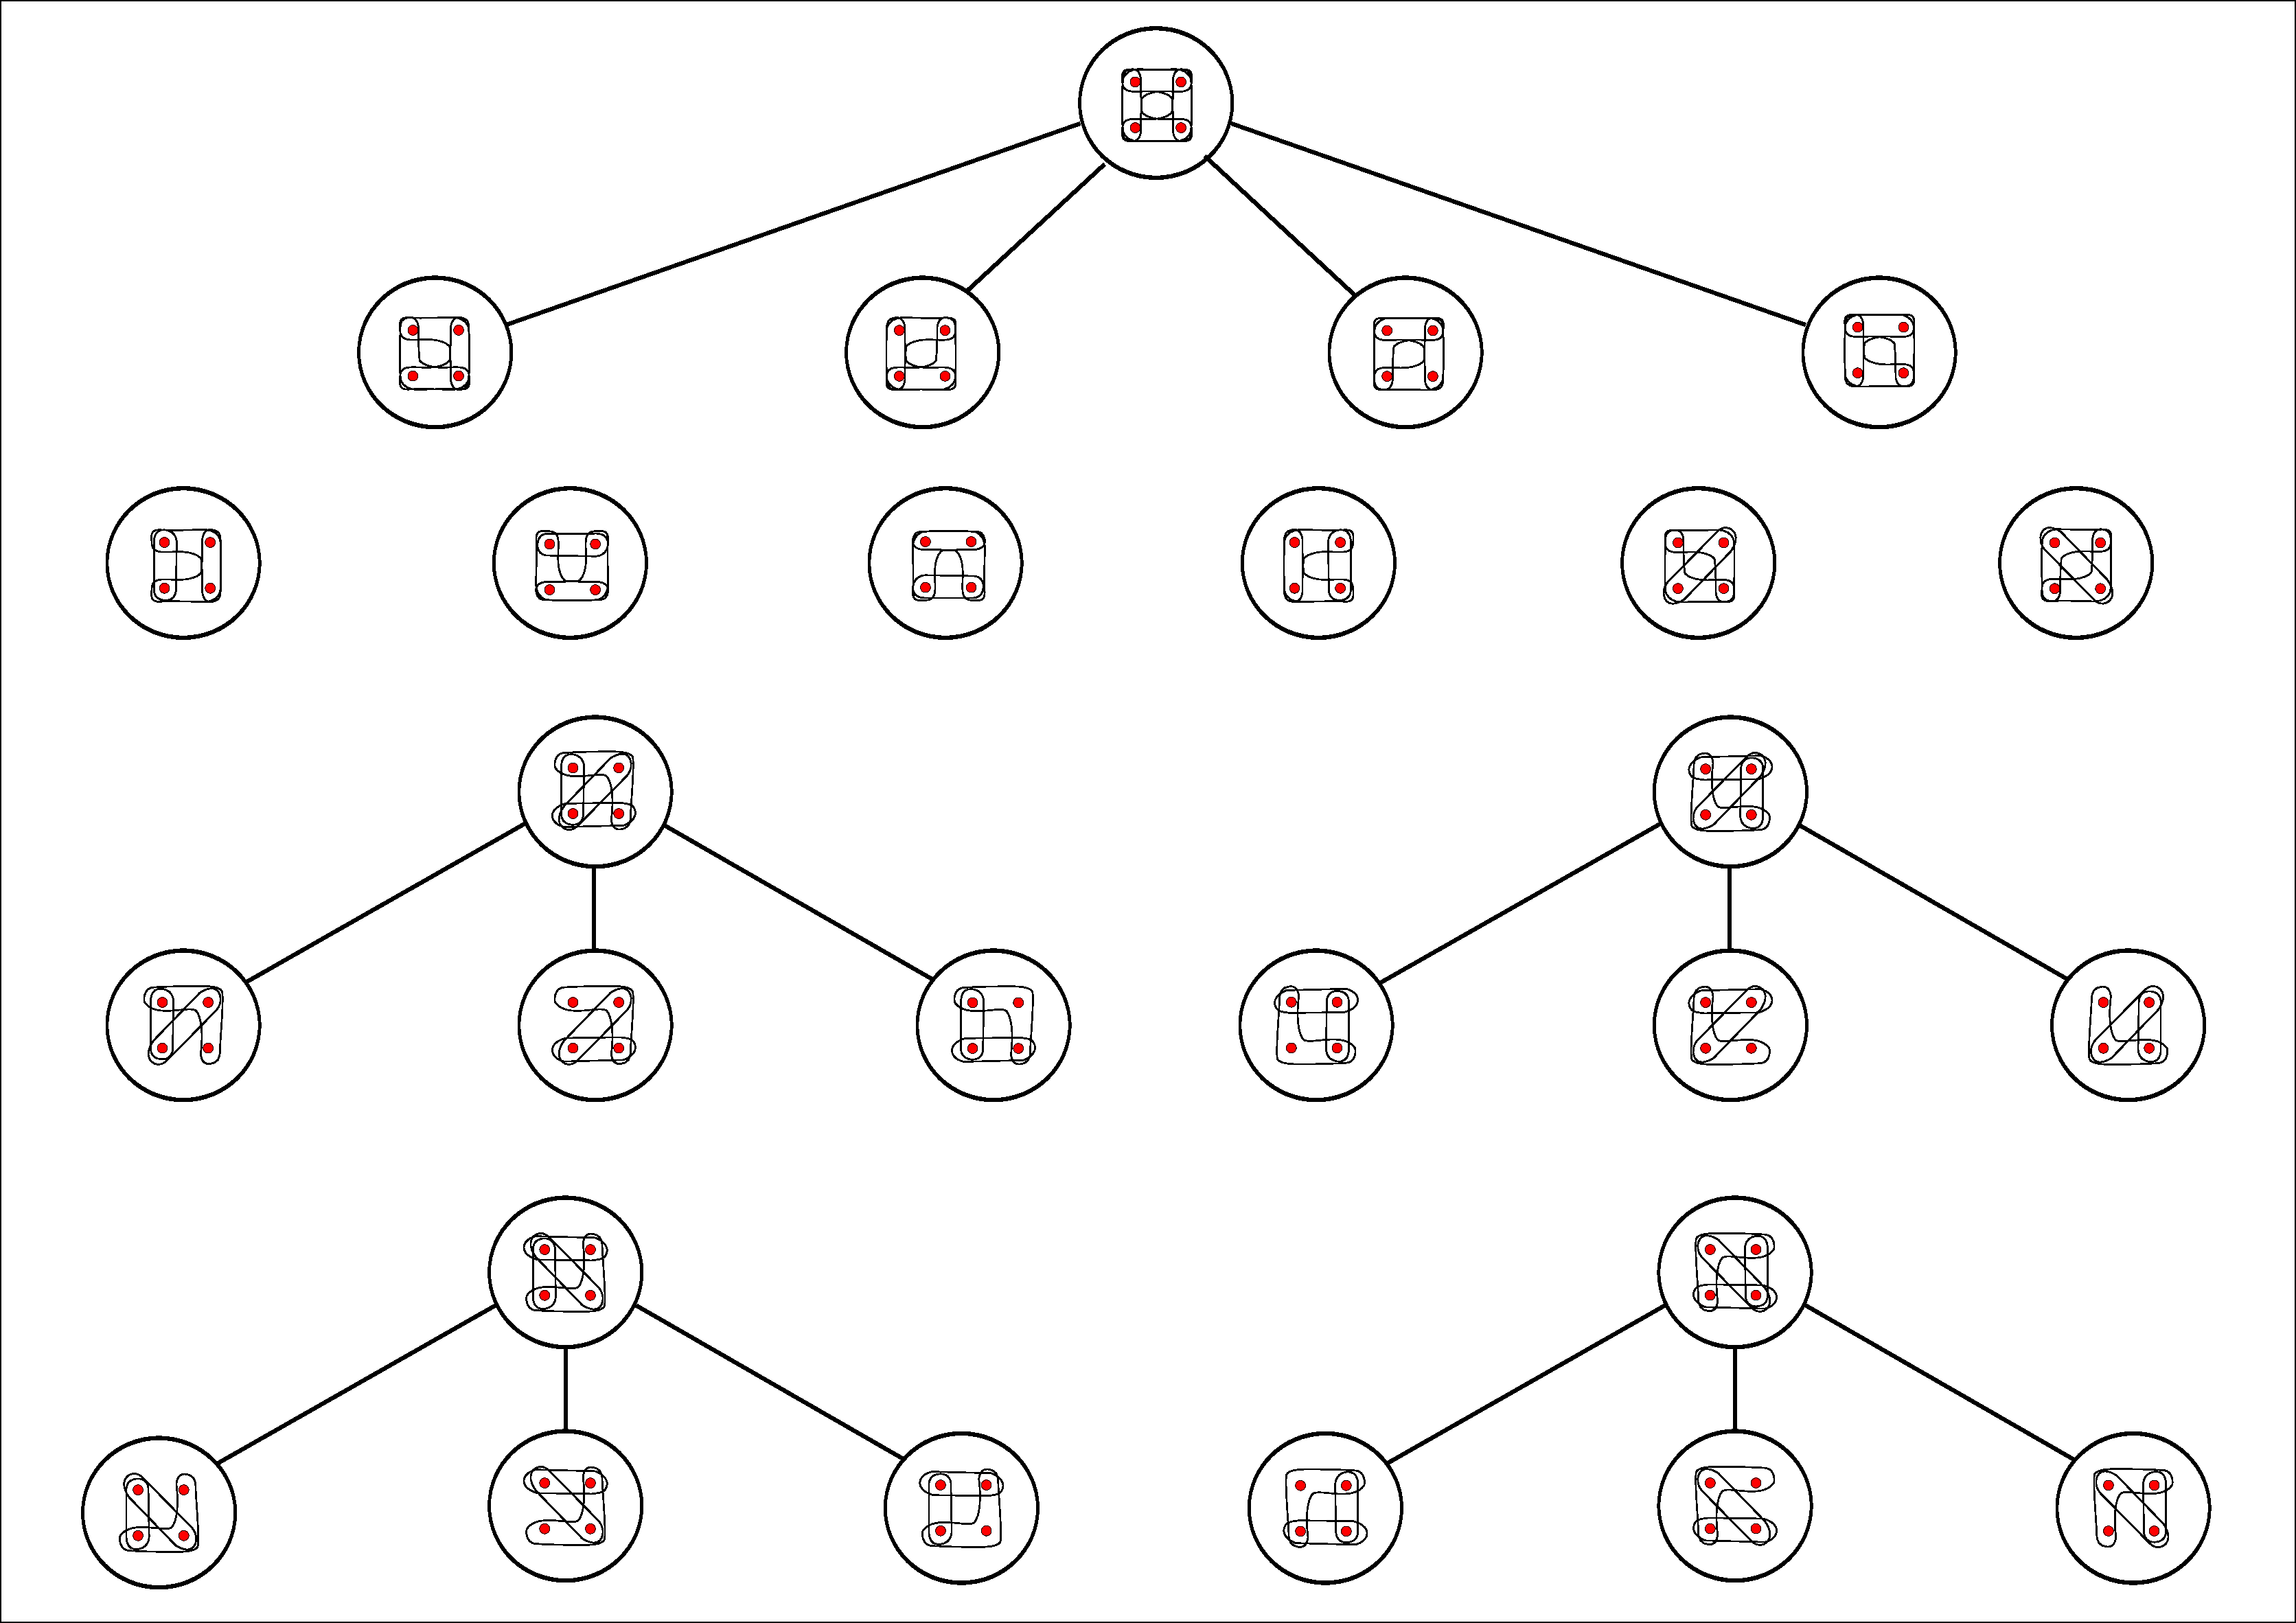
\includegraphics[width=1.0\columnwidth]{fig/non2uniformcyclichypergraphhasse.pdf}
\caption{{\bf Hierarchical relationships among all possible classes of hypergraphs that are not graphs (i.e. not 2-uniform) but have cycles.} (A) There is a Hasse diagram for the lattice of GRNAs analogous to that of \ref{fig:conediagram}A but defined on four rather than only three genes. Within this lattice some of the graphs have cycles and some do not. (B) The highest levels of the Hasse diagram associated to the lattice of GRNAs on four genes containing hypergraphs having cycles. (C) and (D) contain lower levels of GRNAs containing cycles. Each of the four panels in (D) are on the same level. In total, each level represents an isomorphism class of hypergraphs. Therefore, there are five isomorphism classes of non-2-uniform hypergraphs representing GRNAs on four genes that contain cycles leading to the relationship between spaces of probability distsributions on associated genotype-phentoype maps analogous to that of \ref{fig:conediagram}C.}
\label{fig:non2uniformcyclichypergraphhasse}
\end{figure}

\begin{figure}[!ht]
\centering
\noindent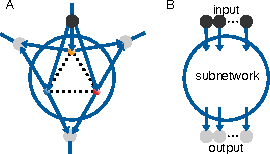
\includegraphics[width=0.3\columnwidth]{fig/controlnetwork.pdf}
\caption{{\bf Embedding into a particular network context.} The network inside the blue circle is equivalent to that of \ref{fig:inconsistentthreecycle}A, embedded into a particular network context that provides inputs (dark gray node) and outputs (light gray nodes) to the focal subnetwork. As a result of their connectivity, the outputs depend here upon pairwise correlations within the three genes comprising the focal subnetwork.}
\label{fig:controlnetwork}
\end{figure}
